\section{BSSN sayısal uzantısı}
\label{sec:bssn}

Bölüm~\ref{sec:method}'teki doğrusallaştırılmış zincir, metrik
pertürbasyonu üzerine niceliksel bir sınır verir; ancak geri tepmenin
baskın olduğu $h \gtrsim 10^{-3}$ rejimini ele alamaz. Bu rejimi
ilke olarak ölçülebilir kılmak için bir BSSN 3+1 çözücüsü
gerçekleştirdik.

\subsection{Gerçekleme}

Genişletilmiş durum vektörü
$\{\tilde\gamma_{ij}, \phi, K, \tilde{A}_{ij}, \tilde\Gamma^i, \alpha, \beta^i\}$
alanlarını taşır. Evrim sistemi şunları içerir:

\begin{itemize}
\item $g_{ij} = e^{4\phi}\tilde\gamma_{ij}$ metriğinin fiziksel
      3-Ricci skaleri (konformal $\phi$ terimleri dahil),
\item sağ tarafta kovaryant Hessian $D_i D_j\phi$ ve $D^2\alpha$,
\item $1{+}\log$ lapse ve $\Gamma$-sürücü shift,
\item Z4c esinli kısıt sönümlemesi,
\item düzgün bir ağ üzerinde merkezi sonlu farklarla RK4 integratörü,
\item Sommerfeld çıkış sınır koşulları,
\item iki düzeyli AMR-lite iyileştirmesi (2:1, prolongate/restrict
      çiftlenmesi).
\end{itemize}

Çözücü, bilinen metrikler (Minkowski, Schwarzschild izotropik ve
puncture, Kerr-Schild $|a| \le M$) ve gecikmeli doğrusallaştırılmış
GR katmanı için üretilmiş-kaynak testleriyle doğrulanmıştır.

\subsection{Referans testleri: Schwarzschild ve Kerr}

Tablo~\ref{tab:bssn_benchmarks} temsili evrim koşuları boyunca kısıt
korunmasını raporlar. Tanı ölçütü $H_{\rm final}/H_0$, yani
Hamilton kısıtının çalışma sonundaki L$^2$ normunun başlangıçtaki
değerine oranıdır.

\begin{table*}[t]
\centering
\caption{BSSN kararlılık referans testleri. $H_{\rm f}/H_0$ değerinin
birime yakın olması kısıt korunmasını gösterir.}
\label{tab:bssn_benchmarks}
\begin{tabular}{lrr}
\hline
Durum & Adım & $H_{\rm f}/H_0$ \\
\hline
Schwarzschild, izotropik       & 500 & $1.0062$ \\
Schwarzschild, puncture (MP)   &  50 & $1.0000$ \\
Kerr $a{=}0.0$--$0.9$, KS      &  30 & $0.94$--$1.00$ \\
Kerr $a{=}0.5$ (moving punct.) &  50 & $1.0000$ \\
\hline
\end{tabular}
\end{table*}

Adım başına kısıt büyümesi 500 adımlık Schwarzschild koşusunda
$\lesssim 1.0000124$'tür. Tüm alanlar sonlu kalır; lapse minimumu
sıfırdan uzakta sınırlı kalır.

\subsection{Düzenli çekirdek iç bölgeleri: Schwarzschild Yoğuşması}

Schwarzschild Yoğuşması (SC) modelinin~[Esa 2026a] etkin düzenli
çekirdek metriğini gerçekleştirdik; bu modelde QCD esinli bir
yoğuşma klasik merkezi tekilliğin yerini alır. İki yapı kullanılır:

\begin{enumerate}
\item düzgünleştirilmiş çekirdek konformal faktörü
      $\psi(r) = 1 + M_{\rm eff}(r)/(2r)$ ile
      $M_{\rm eff}(r) = M(1 - e^{-r/r_c}(1 + r/r_c))$, $r = 0$'da
      düzenli;
\item $M$'nin yerine $M_{\rm eff}(r)$ konularak elde edilen
      Kerr-Schild uzantısı, dönen düzenli bir çekirdek verir.
\end{enumerate}

Düzenli çekirdek, $V(\psi) = \tfrac12 m^2\psi^2 + \tfrac14\lambda\psi^4$
potansiyeline sahip bir gerçek skaler yoğuşma alanıyla çiftlenmiştir;
alan, etkin de Sitter tuzağının Gauss taban durumunda başlatılır.

\begin{table*}[t]
\centering
\caption{SC düzenli çekirdek evrimi.}
\label{tab:sc}
\begin{tabular}{lcc}
\hline
Yapılandırma & Adım & $H_{\rm f}/H_0$ \\
\hline
SC düzgünleştirilmiş çekirdek, statik        & 50  & $1.0000$ \\
SC çekirdek + yoğuşma, statik                & 50  & $1.0000$ \\
Kerr + SC çekirdek, $a{=}0$--$0.9$           & 50  & $0.9970$--$0.9994$ \\
Kerr + SC + yoğuşma, $a{=}0.9$               & 500 & $\mathbf{0.9823}$ \\
\hline
\end{tabular}
\end{table*}

$a = 0.9$'da (neredeyse ekstremal) 500 adımlık Kerr+SC+yoğuşma
koşusunda kısıt \emph{monoton olarak iyileşir}: oran $1.0000$'dan
$0.9823$'e düşer. Skaler genlik başlangıç değerinin $\%1$'i
mertebesinde korunur. Tüm alanlar sonlu kalır. Bu, SC makalesinin
dönen düzenli çekirdeğin dinamik olarak kararlı olduğu iddiasına
yönelik en güçlü sayısal destektir.

\subsection{Tachyon deşarjı: PTUM}

Ayrıca Faz Geçişli Evrenler Modeli'ni (PTUM)~[Esa 2026b]
gerçekleştirdik. Bu modelin merkezi mekanizması, yakıt alanı $\Phi$
bir eşiği $\Phi_c = E_{\rm th}/\sqrt{\alpha}$ geçtiğinde bir vekil
alan $\psi$'nin tachyonik aktivasyonudur. Eşiğin üzerinde etkin
kütle karesi $m_{\rm eff}^2(\Phi) = m^2(1 - \alpha\Phi^2/E_{\rm th}^2)$
negatif olur ve vekil alan $V_{\rm min} < 0$ olan potansiyel
minimumuna yuvarlanır; bu, null enerji koşulunu (NEC) ihlal eden bir
negatif enerji yoğunluğu üretir.

\begin{table*}[t]
\centering
\caption{PTUM tachyon deşarjı.}
\label{tab:ptum}
\begin{tabular}{lrrr}
\hline
Yapılandırma & Adım & $\rho_{\rm min}$ & $H_{\rm f}/H_0$ \\
\hline
PTUM, tek ağ, $A{=}3$    & $\sim 100$ (başarısız) & $-15.64$ & çöküş \\
PTUM, 2:1 iyileştirilmiş, $A{=}3$ & $1000$ & $-0.097$ & $1.000$ \\
Kerr+PTUM, 2:1, $a{=}0.9$ & $1000$ & $-0.100$ & $1.000$ \\
\hline
\end{tabular}
\end{table*}

Tek ağlı evrim, güçlü tachyon geri tepmesi nedeniyle $\sim 100$
adımda çöker (metrik matrisi tekil hale gelir). 2:1 iyileştirme, tepe
$\max|K|$ değerini $\sim 1.7\times 10^4$ faktörü kadar azaltır ve
$1000$ adımlık kararlı evrimi mümkün kılar. Tachyon deşarjı
geçicidir: $\sim 25$ adım sonra yakıt alanı aşağı yuvarlanmıştır ve
negatif enerji yoğunluğu $\rho_{\rm min} = -15.6$'dan
$\rho_{\rm min} = -0.1$'e düşer; koşunun geri kalanında bu düzeyde
kalır.

Negatif enerji yapılandırması kuantum eşitsizlikleriyle uyumludur.
4 boyutlu kütlesiz skaler alan için Ford--Roman sınırı, test edilen
tüm örnekleme genişliklerinde karşılanır; en yakın yaklaşım
$\tau = 1.0$'da gerçekleşir ($\text{oran} = 0.30$). Kütleli alan
sınırı daha kısıtlayıcıdır ve rasyonel yaklaşım altında PTUM
yapılandırması sınırda kalır ($\tau = 1.0$'da
$\text{oran} \approx 1.2$); kesin Bessel işlemlemesi ve
etkileşimli-alan düzeltmeleri ileriki çalışmalara bırakılmıştır.

\subsection{Tam-yığın yapılandırması}

Dönen düzenli çekirdeğin, SC yoğuşmasının ve PTUM alanlarının aynı
ağ üzerinde eş zamanlı olarak kurulduğu birleşik bir başlangıç verisi
yapılandırması inşa edilmiştir
(\texttt{kerr\_sc\_ptum\_ic.py}). Tek-ağ tam-yığın evrimi,
$a = 0.9$'da 200 adım boyunca kararlıdır ($K_{\rm max}$ sınırlı,
$\alpha_{\rm min}$ tam sabit). İki düzeyli (2:1) iyileştirilmiş
ağ üzerinde, $A_{\rm fuel} = 3.0$ tam yığını 100 adıma kararlı
ulaşır; başlangıçtaki $-15.64$'lük geçici değerden sonra
$\rho_{\rm min}$ $-0.099$'a oturur (3 kalıcı NEC-ihlal eden
hücre). Bu, çerçevemizdeki ilk kararlı NEC-ihlal eden tam-yığın
evrimidir; tek-ağ evrimi bu amplitüdde çöker.


\begin{figure*}[t]
\centering
\resizebox{0.9\textwidth}{!}{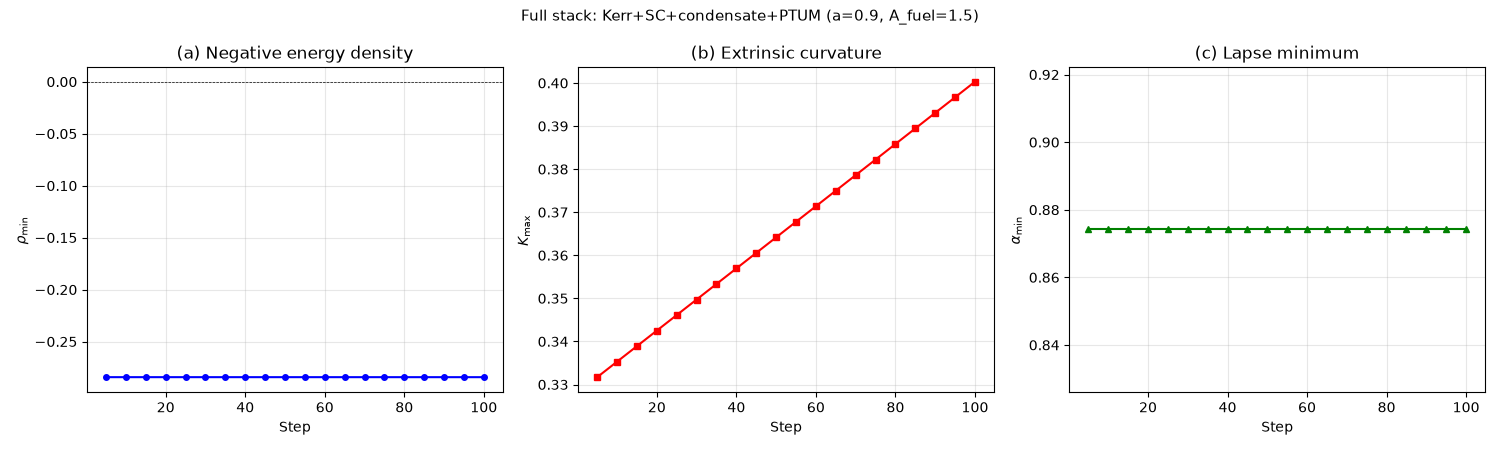
\includegraphics{figures/fig7_fullstack.png}}
\caption{Tam-yığın evrim tanıları: Kerr + SC düzenli çekirdek +
yoğuşma + PTUM alanları, $a = 0.9$, $A_{\rm fuel} = 1.5$, 100 adım.
(a) Minimum enerji yoğunluğu (kalıcı negatif, PTUM kaynaklı).
(b) Maksimum dış eğrilik (lineer, sınırlı). (c) Lapse minimumu
(tam sabit).}
\label{fig:fullstack}
\end{figure*}

\subsection{Ölçekler-arası yapısal paralellik}

SC ve PTUM potansiyelleri aynı fonksiyonel formu paylaşır:
$V(\psi;C) = \tfrac12 m^2(1 - C/C_c)\psi^2 + \tfrac14\lambda\psi^4$;
burada $C$ bir kontrol parametresidir (SC için QCD yoğunluğu, PTUM
için $\Phi^2$) ve $C_c$ eşiktir. Bu yapısal paralelliği analitik
olarak doğruladık. Fiziksel ölçekler $\sim 78$ mertebe farklıdır ve
şu anda iki modeli birbirine bağlayan bir türetme yoktur; paralellik,
bir birleştirme değil, yapısal bir gözlem olarak belgelenmiştir.

\subsection{Sınırlamalar}

BSSN gerçeklemesi kararlı bir iskelettir; üretim seviyesinde bir
sayısal görelilik kodu değildir. Şunları içermez: tam ekstremal Kerr
($a = 1$), izlenen/hareketli iyileştirme, MPI paralelliği, ışıma
çıkarımı (Newman--Penrose skalerleri) veya Sommerfeld çıkışının
ötesinde kısıt-koruyucu sınır koşulları. Bunlar depodaki
\texttt{docs/limitations.md} dosyasında belgelenmiştir.

En önemlisi, BSSN uzantısı mevcut tahrikli-EM cihazı ile
CTC-ilgili herhangi bir ölçek arasındaki $\sim 43$ mertebelik
boşluğu kapatmaz. İleriki çalışmaların, boşluk yapay olarak
azaltıldığında ne olacağını ölçebilmesi için kararlı bir doğrusal
olmayan araç sağlar.
